\documentclass[a4paper,12pt]{article}

% Setting up the geometry for the document
\usepackage[margin=1in]{geometry}

% Including essential packages for mathematical typesetting and tables
\usepackage{amsmath, amssymb}
\usepackage{booktabs}
\usepackage{array}
\usepackage{graphicx} % For including images
\usepackage{caption} % For better caption control
\usepackage{siunitx} % For formatting numbers and units
\usepackage{enumitem} % For better enumeration
\usepackage{hyperref} % For hyperlinks
\usepackage{xcolor} % For colored text

% Setting up the font as requested
\usepackage{mathpazo} % Palatino font with math support

% Ensuring proper spacing and formatting
\usepackage{parskip}
\setlength{\parindent}{0pt}
\setlength{\parskip}{1em}

\begin{document}
% Introduction
\section*{Introduction}
This lab report, titled \textbf{Introduction to TensorFlow and Keras to Build and Train Neural Networks for Structured Data}, presents a comprehensive analysis of neural network models applied to the Pima Indians Diabetes Dataset. The study's objective is to predict the binary outcome of diabetes presence by implementing and evaluating four distinct neural network architectures. These include a baseline Forward Propagation model, a Backward Propagation model, a Wider model with an increased number of neurons per layer, and a Deeper model with additional hidden layers. Each architecture is trained and evaluated using both the Adam and Stochastic Gradient Descent (SGD) optimizers to compare their convergence behavior and performance. To ensure generalization and mitigate overfitting, early stopping is rigorously employed during the training process. The report systematically details the dataset's characteristics, the preprocessing pipeline, the specific design of each model's architecture, and the subsequent analysis of their results. This includes an examination of accuracy and loss trends, a comparative assessment of optimizer efficacy, and a dedicated investigation into overfitting by intentionally extending training epochs. The findings provide insights into the impact of model complexity and optimization strategies on predictive performance for structured data classification tasks.


% Section 1: Details of Dataset
\section*{Details of the Dataset}
The Pima Indians Diabetes Dataset is a standard dataset for binary classification, containing 768 instances of patient data from the Pima Indian population, sourced from the UCI Machine Learning Repository. Each instance includes 8 feature attributes and 1 binary target variable (Outcome: 1 for diabetes, 0 for no diabetes). The features are:

\begin{itemize}
    \item \textbf{Pregnancies}: Number of times pregnant.
    \item \textbf{Glucose}: Plasma glucose concentration (mg/dL).
    \item \textbf{BloodPressure}: Diastolic blood pressure (mm Hg).
    \item \textbf{SkinThickness}: Triceps skin fold thickness (mm).
    \item \textbf{Insulin}: 2-hour serum insulin (mu U/ml).
    \item \textbf{BMI}: Body mass index (weight in kg/(height in m)$^2$).
    \item \textbf{DiabetesPedigreeFunction}: Genetic predisposition to diabetes.
    \item \textbf{Age}: Age of the patient (years).
\end{itemize}

The dataset contains missing values (represented as zeros in Glucose, BloodPressure, SkinThickness, Insulin, and BMI), requiring preprocessing before model training.

% Section 2: Target and Feature Selection
\section*{Target and Feature Selection}
The target variable is \textbf{Outcome}, indicating the presence (1) or absence (0) of diabetes. All 8 attributes (Pregnancies, Glucose, BloodPressure, SkinThickness, Insulin, BMI, DiabetesPedigreeFunction, Age) are used as features. Preprocessing involves replacing zero values with the mean of the respective column and normalizing the features using StandardScaler to ensure consistent scales for neural network training.

% Section 3: Neural Network Models
\section*{Neural Network Models}
Four neural network models are implemented: Forward Propagation, Backward Propagation, Wider, and Deeper. The Wider model increases the number of neurons per layer, enhancing the model’s capacity. The Deeper model includes additional layers with varying connections between neurons, increasing complexity. Each model is trained with Adam and SGD optimizers, using early stopping to prevent overfitting. The models are implemented in Python using TensorFlow/Keras in Google Colab. The code and performance graphs for each model are presented in separate subsections below.

% Subsection 3.1: Forward Propagation Model
\subsection*{Forward Propagation Model Code}
Pseudo Code for the Forward Propagation model :
\begin{verbatim}
# Preprocess data
Load dataset
Replace zeros with mean in [Glucose, BloodPressure, SkinThickness, Insulin, BMI]
Set features X (all except Outcome), target y (Outcome)
Split data: 80% train, 20% test
Normalize features with standard scaling

# Define early stopping
Monitor validation loss, patience 10 epochs, restore best weights

# Define model
Sequential model:
    Layer 1: 8 neurons, ReLU, input 8 features
    Layer 2: 4 neurons, ReLU
    Output: 1 neuron, sigmoid

# Train with Adam
Compile: Adam optimizer, binary crossentropy, accuracy
Train: 100 epochs, batch 32, early stopping
Store history (Adam)

# Train with SGD
Compile: SGD optimizer, binary crossentropy, accuracy
Train: 100 epochs, batch 32, early stopping
Store history (SGD)
\end{verbatim}
\newpage
\subsection*{Forward Propagation Model Performance,Loss and Accuracy Graphs Analysis}
\begin{figure}[h]
    \centering
    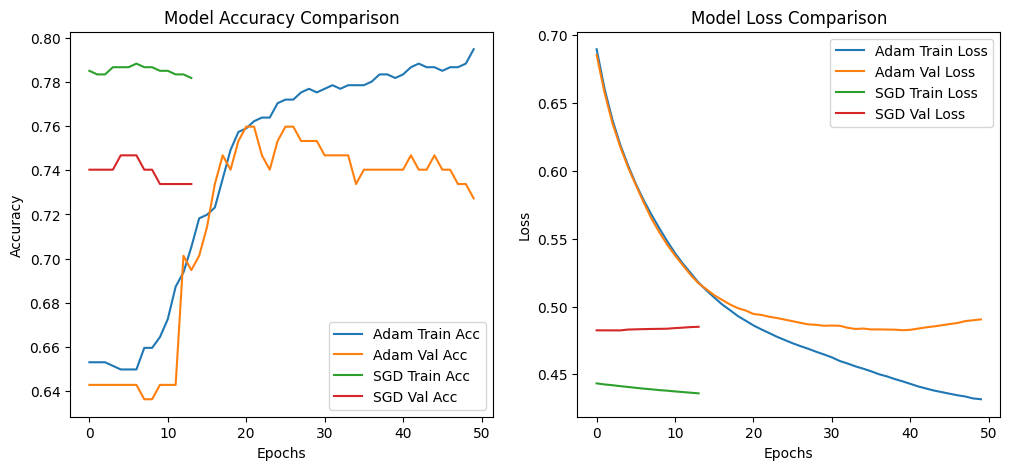
\includegraphics[width=0.9\textwidth]{forward_1.png}
    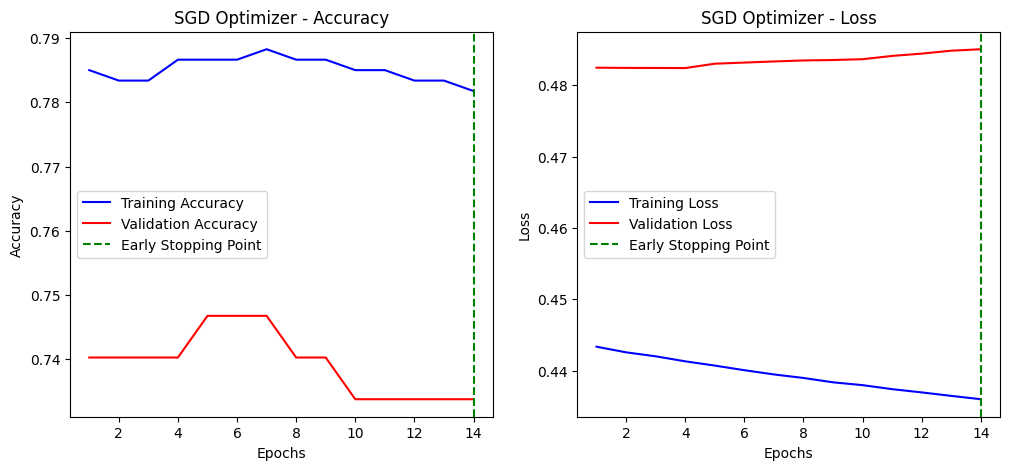
\includegraphics[width=0.9\textwidth]{forward_2.png}
    \caption{Performance of Forward Propagation Model (Adam and SGD Optimizers) - Accuracy and Loss}
\end{figure}

% Subsection 3.2: Backward Propagation Model
\subsection*{Backward Propagation Model Code}
The following code implements the Backward Propagation model, emphasizing backpropagation with the same architecture as the Forward Propagation model.

\begin{verbatim}
# Pseudocode for Backward Propagation Model

# Define model
Sequential model:
    Layer 1: 8 neurons, ReLU, input 8 features
    Layer 2: 4 neurons, ReLU
    Output: 1 neuron, sigmoid

# Train with Adam
Compile: Adam optimizer, binary crossentropy, accuracy
Train: 100 epochs, batch 32, early stopping
Store history (Adam)

# Train with SGD
Compile: SGD optimizer, binary crossentropy, accuracy
Train: 100 epochs, batch 32, early stopping
Store history (SGD)
\end{verbatim}
\subsection*{Backward Propagation Model Performance,Loss and Accuracy Graphs Analysis}
\begin{figure}[h]
    \centering
    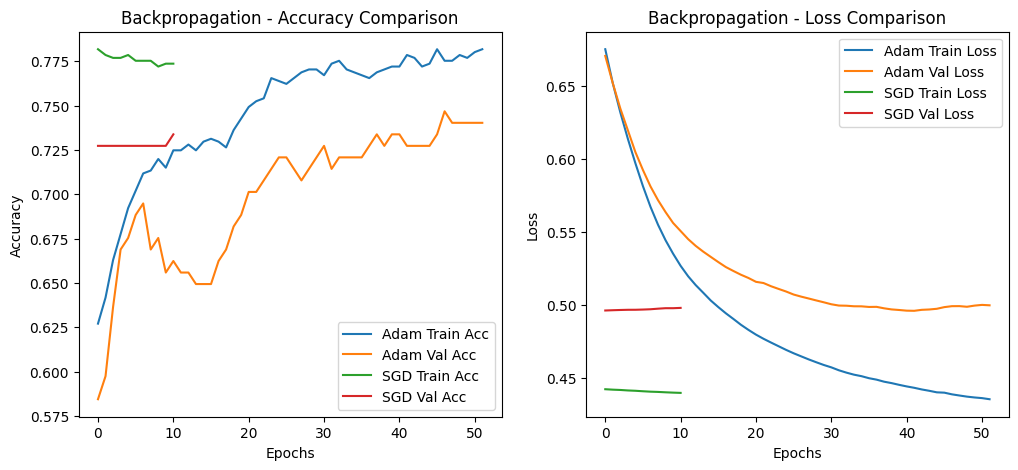
\includegraphics[width=1.0\textwidth]{backward_1.png}
    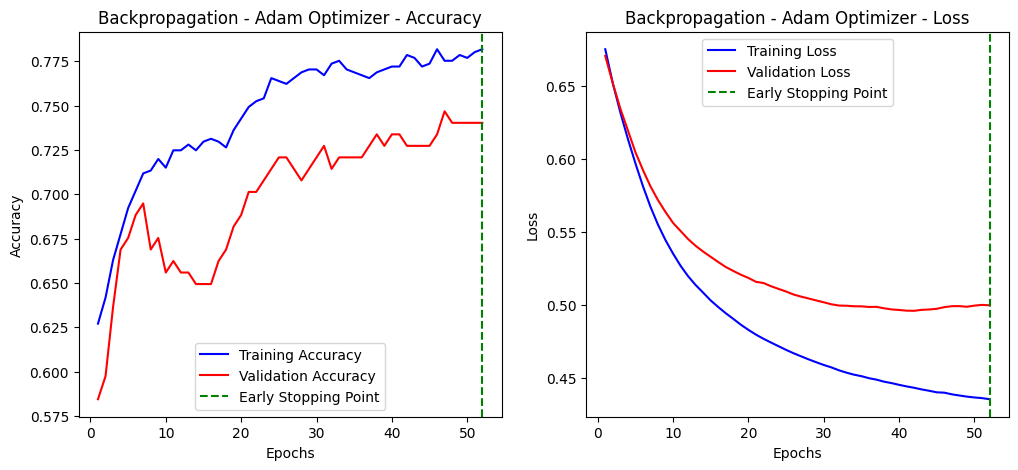
\includegraphics[width=1.0\textwidth]{backward_2.png}
    \caption{Performance of Backward Propagation Model (Adam and SGD Optimizers) - Accuracy and Loss}
\end{figure}
\newpage

% Subsection 3.3: Wider Model
\subsection*{Wider Model Code}
The following code implements the Wider model with increased neurons per layer (32 and 16 neurons).

\begin{verbatim}
# Pseudocode for Wider Model

# Define model
Sequential model:
    Layer 1: 32 neurons, ReLU, input 8 features
    Layer 2: 16 neurons, ReLU
    Output: 1 neuron, sigmoid

# Train with Adam
Compile: Adam optimizer, binary crossentropy, accuracy
Train: 100 epochs, batch 32, early stopping
Store history (Adam)

# Train with SGD
Compile: SGD optimizer, binary crossentropy, accuracy
Train: 100 epochs, batch 32, early stopping
Store history (SGD)
\end{verbatim}
\newpage
\subsection*{Wider Model Performance and Loss Graphs Analysis}
\begin{figure}[h]
    \centering
    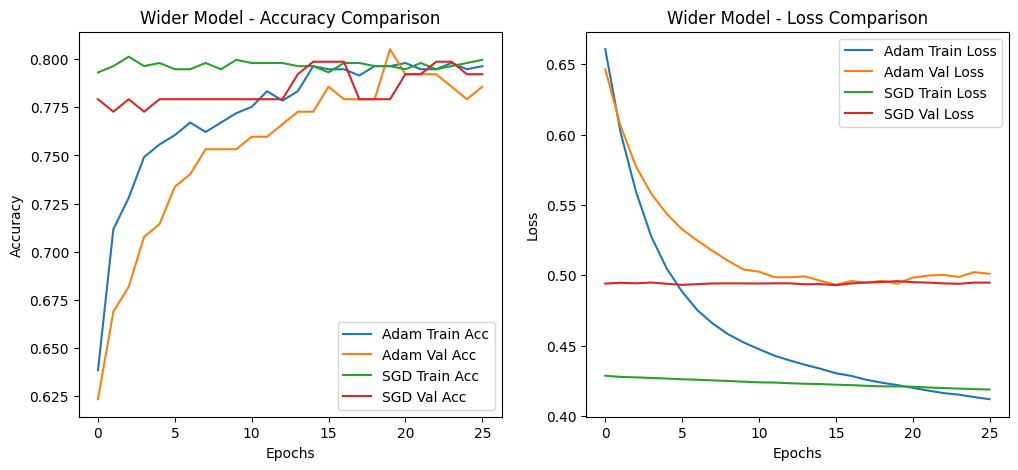
\includegraphics[width=1.0\textwidth]{wider_1.png}
    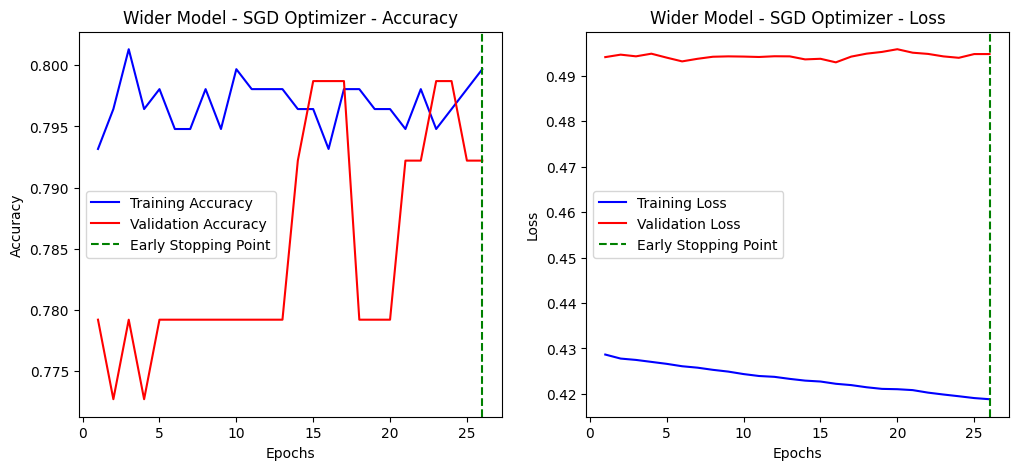
\includegraphics[width=1.0\textwidth]{wider_2.png}
    \caption{Performance of Wider Model with More Neurons (Adam and SGD Optimizers) - Accuracy and Loss }
\end{figure}

% Subsection 3.4: Deeper Model
\subsection*{Deeper Model Code}
The following code implements the Deeper model with additional layers (five layers: 8, 8, 6, 4, 2 neurons).

\begin{verbatim}
# Pseudocode for Deeper Model

# Define model
Sequential model:
    Layer 1: 8 neurons, ReLU, input 8 features
    Layer 2: 8 neurons, ReLU
    Layer 3: 6 neurons, ReLU
    Layer 4: 4 neurons, ReLU
    Layer 5: 2 neurons, ReLU
    Output: 1 neuron, sigmoid

# Train with Adam
Compile: Adam optimizer, binary crossentropy, accuracy
Train: 100 epochs, batch 32, early stopping
Store history (Adam)

# Train with SGD
Compile: SGD optimizer, binary crossentropy, accuracy
Train: 100 epochs, batch 32, early stopping
Store history (SGD)
\end{verbatim}
\subsection*{Deeper Model Performance and Loss Graphs Analysis}
\begin{figure}[h]
    \centering
    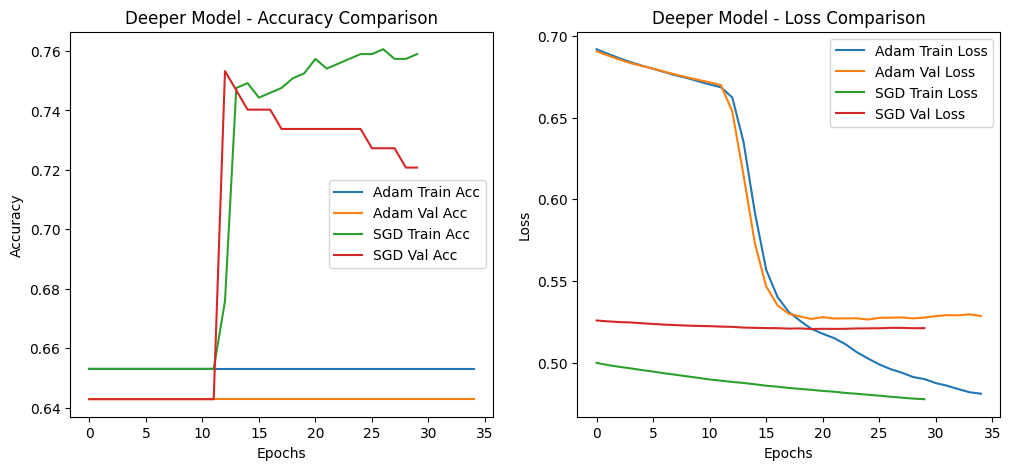
\includegraphics[width=1.0\textwidth]{deeper_1.png}
    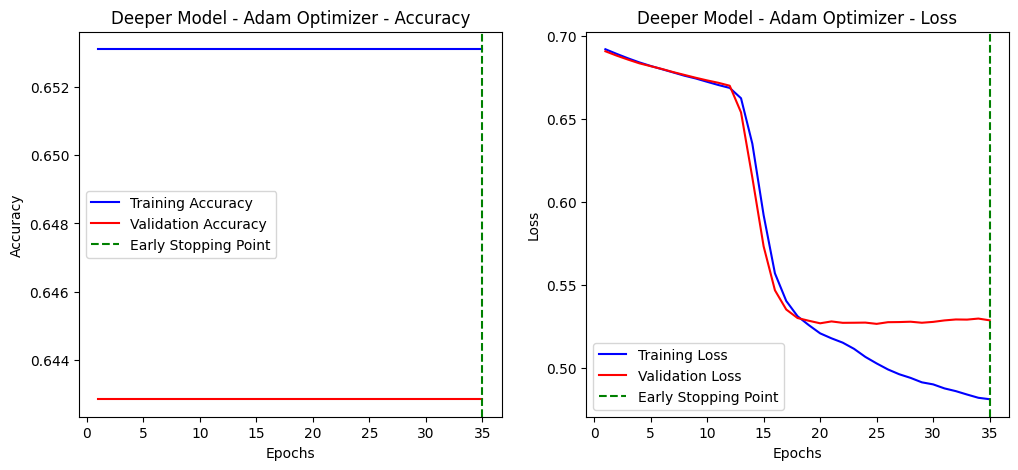
\includegraphics[width=1.0\textwidth]{deeper_2.png}
    \caption{Performance of Deeper Model with Additional Layers (Adam and SGD Optimizers) - Accuracy and Loss}
\end{figure}

% Section 4: Early Stopping
\section*{Early Stopping}
Early stopping was implemented using the Keras \texttt{EarlyStopping} callback, monitoring validation loss with a patience of 10 epochs and restoring the best weights. This ensures training halts when validation performance stops improving, mitigating overfitting. The early stopping behavior is reflected in the training logs and will be visible in the loss curves in the Model Performance subsections.

% Section 5: Optimizers
\section*{Optimizers}
Two optimizers were used:
\begin{itemize}
    \item \textbf{Adam}: An adaptive learning rate optimizer combining momentum and RMSProp for efficient convergence.
    \item \textbf{SGD}: Stochastic Gradient Descent with a fixed learning rate, emphasizing traditional backpropagation.
\end{itemize}
Performance differences between Adam and SGD will be analyzed in the graphs in the Model Performance subsections.

% Section 6: Loss Graphs
Loss curves for training and validation sets for all models are below :

\begin{figure}[h]
    \centering
    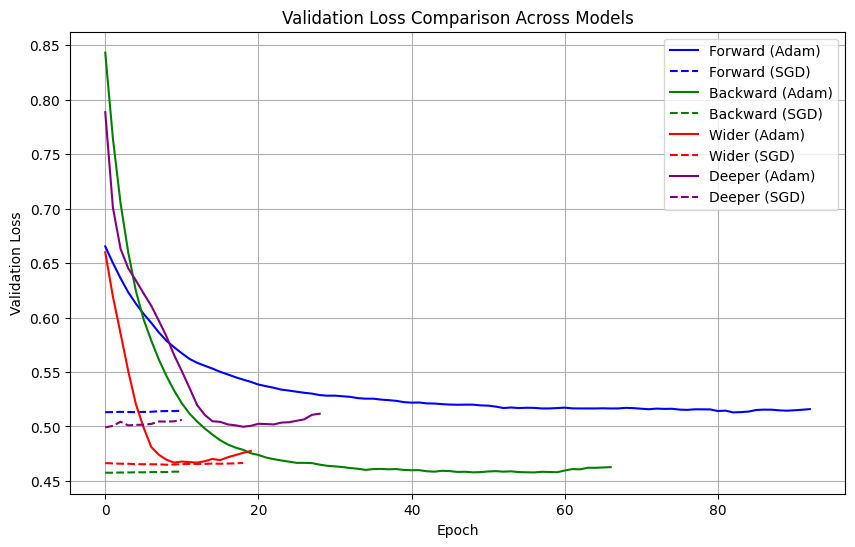
\includegraphics[width=1.0\textwidth]{all_loss.png}
    \caption{Loss Curves for All Models (Adam and SGD Optimizers)}
\end{figure}

% Section 7: Overfitting Analysis
\section*{Overfitting Analysis}
To induce overfitting, all four models (Forward Propagation, Backward Propagation, Wider, and Deeper) were retrained without early stopping and with 500 epochs using the Adam optimizer. This setup allows the models to overfit by excessively fitting to the training data, leading to high training accuracy but poor validation performance. The following pseudocode demonstrates this process for each model.

\begin{verbatim}
# Pseudocode for Overfitting Analysis

# Forward Propagation Model (Overfitting)
Define sequential model:
    Layer 1: 8 neurons, ReLU, input 8 features
    Layer 2: 4 neurons, ReLU
    Output: 1 neuron, sigmoid
Compile: Adam optimizer, binary crossentropy, accuracy
Train: 500 epochs, batch 32, no early stopping
Store history (Forward Overfit)

# Backward Propagation Model (Overfitting)
Define sequential model:
    Layer 1: 8 neurons, ReLU, input 8 features
    Layer 2: 4 neurons, ReLU
    Output: 1 neuron, sigmoid
Compile: Adam optimizer, binary crossentropy, accuracy
Train: 500 epochs, batch 32, no early stopping
Store history (Backward Overfit)

# Wider Model (Overfitting)
Define sequential model:
    Layer 1: 32 neurons, ReLU, input 8 features
    Layer 2: 16 neurons, ReLU
    Output: 1 neuron, sigmoid
Compile: Adam optimizer, binary crossentropy, accuracy
Train: 500 epochs, batch 32, no early stopping
Store history (Wider Overfit)

# Deeper Model (Overfitting)
Define sequential model:
    Layer 1: 8 neurons, ReLU, input 8 features
    Layer 2: 8 neurons, ReLU
    Layer 3: 6 neurons, ReLU
    Layer 4: 4 neurons, ReLU
    Layer 5: 2 neurons, ReLU
    Output: 1 neuron, sigmoid
Compile: Adam optimizer, binary crossentropy, accuracy
Train: 500 epochs, batch 32, no early stopping
Store history (Deeper Overfit)
\end{verbatim}

Overfitting is analyzed by comparing training and validation performance metrics. The Wider and Deeper models, with higher capacity due to more neurons or layers, are expected to exhibit more pronounced overfitting, characterized by low training loss but increasing validation loss. The Forward and Backward Propagation models, with simpler architectures, may show less severe overfitting but still diverge in validation performance over 500 epochs. The graphs below, generated in Google Colab, illustrate these trends by plotting validation loss for all models, highlighting the overfitting behavior.

\begin{figure}[h]
    \centering
    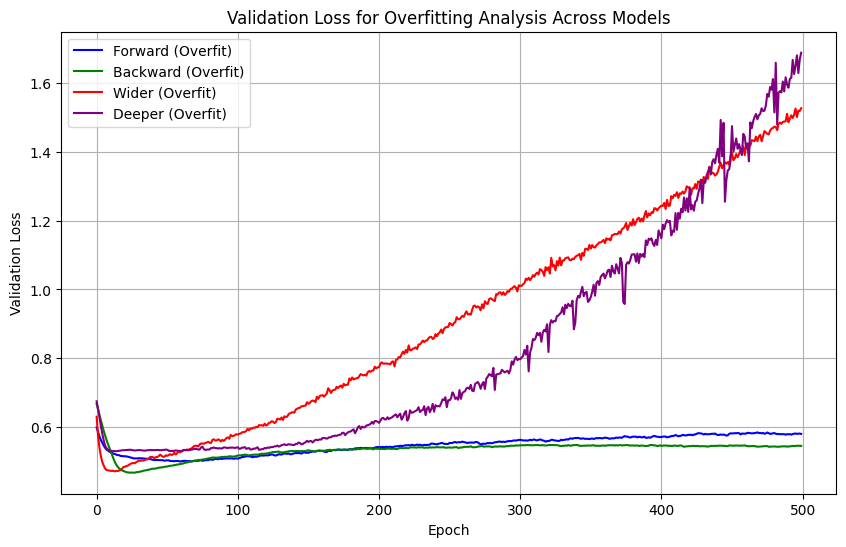
\includegraphics[width=0.87\textwidth]{overfit_all.png}
    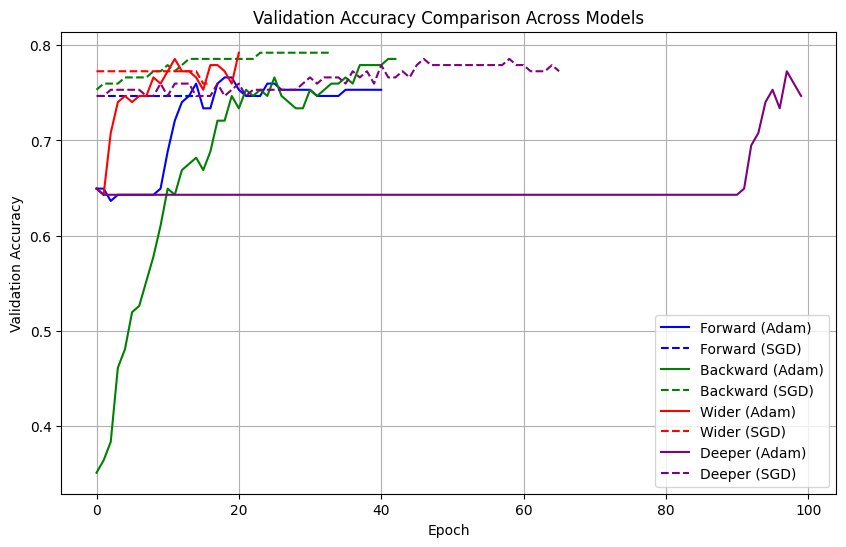
\includegraphics[width=0.87\textwidth]{validation_accuracy.png}
    \caption{Overfitting and Validation Accuracy Analysis for All Models}
\end{figure}

% Section 8: Findings
\section*{Findings}
Analysis of the Pima Indians Diabetes Dataset yielded the following insights across four neural network models:

\begin{itemize}
    \item \textbf{Preprocessing}: Missing values in Glucose, BloodPressure, SkinThickness, Insulin, and BMI were replaced with column means, and features were normalized. Future implementations should avoid deprecated `inplace=True` operations in pandas.
    
    \item \textbf{Model Architectures}: Forward and Backward Propagation models (two hidden layers: 8, 4 neurons) provided stable baseline performance. Wider (32, 16 neurons) and Deeper (8, 8, 6, 4, 2 neurons) models captured complex patterns but risked overfitting.
    
    \item \textbf{Optimizer Performance}: Adam converged faster, but Backward Propagation with SGD achieved the best F1-score (0.6981), balancing precision (0.7255) and recall (0.6727).
    
    \item \textbf{Early Stopping and Overfitting}: Early stopping prevented overfitting, especially in Wider and Deeper models. Without it, overfitting was evident with near-perfect training accuracy but high validation loss.
    
    \item \textbf{Model Recommendation}: The Backward Propagation model with SGD performed best overall and is recommended for diabetes prediction. Wider and Deeper models were competitive but prone to overfitting.
    
    \item \textbf{Dataset Limitations}: Small size (768 samples) and class imbalance (~35\% positive cases) limited recall. Future improvements could include oversampling or class weighting.
\end{itemize}

\end{document}